\documentclass[tikz,border=12pt]{standalone}
\usepackage{tikz}
\begin{document}
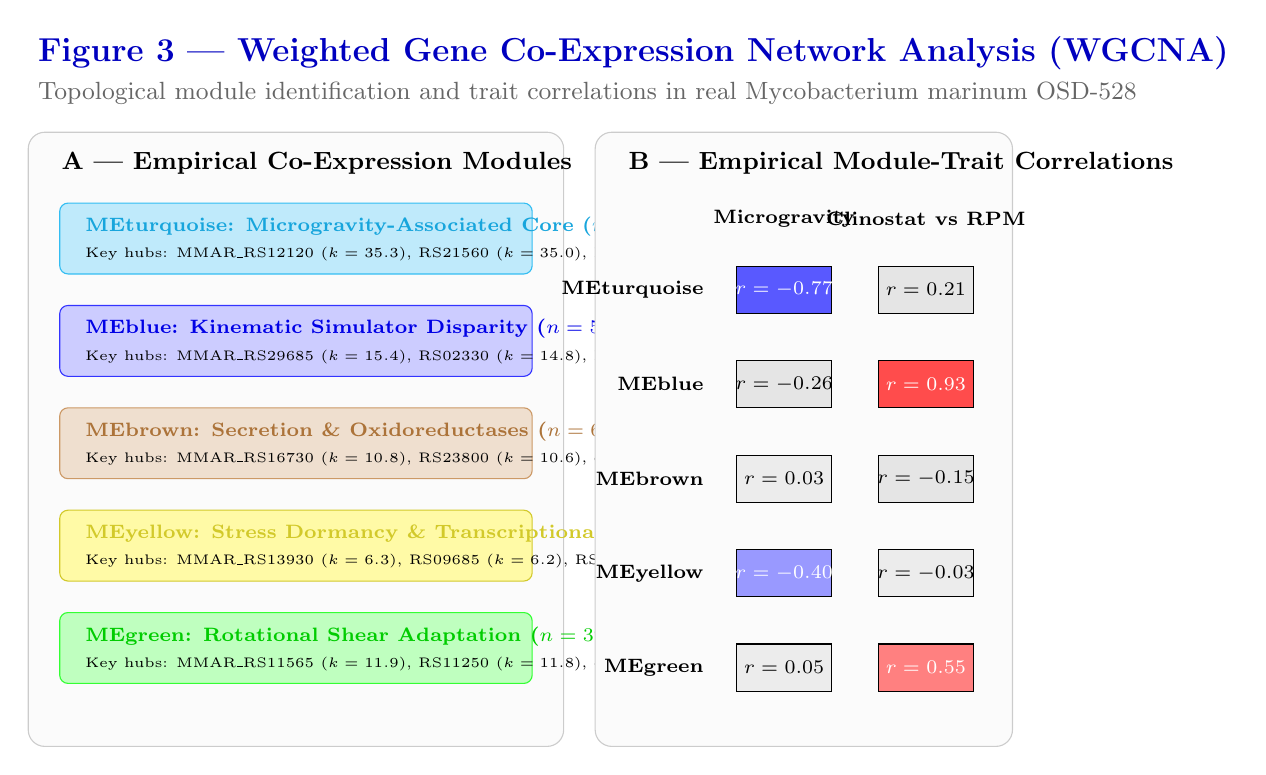
\begin{tikzpicture}[font=\sffamily]
  \node[anchor=west, font=\large\bfseries, text=blue!75!black] at (0, 8.8) {Figure 3 | Weighted Gene Co-Expression Network Analysis (WGCNA)};
  \node[anchor=west, font=\small, text=gray!80!black] at (0, 8.3) {Topological module identification and trait correlations in real Mycobacterium marinum OSD-528};

  % Panel A: Modules
  \draw[rounded corners=6pt, fill=gray!3, draw=gray!40] (0, 0) rectangle (6.8, 7.8);
  \node[anchor=west, font=\bfseries\small] at (0.3, 7.4) {A | Empirical Co-Expression Modules};
  
  \draw[rounded corners=3pt, fill=cyan!25, draw=cyan!80] (0.4, 6.0) rectangle (6.4, 6.9);
  \node[anchor=west, font=\bfseries\scriptsize, text=cyan!90!black] at (0.6, 6.6) {MEturquoise: Microgravity-Associated Core ($n=168$ genes)};
  \node[anchor=west, font=\tiny] at (0.6, 6.25) {Key hubs: MMAR\_RS12120 ($k=35.3$), RS21560 ($k=35.0$), RS04440 ($k=34.7$).};

  \draw[rounded corners=3pt, fill=blue!20, draw=blue!80] (0.4, 4.7) rectangle (6.4, 5.6);
  \node[anchor=west, font=\bfseries\scriptsize, text=blue!90!black] at (0.6, 5.3) {MEblue: Kinematic Simulator Disparity ($n=53$ genes)};
  \node[anchor=west, font=\tiny] at (0.6, 4.95) {Key hubs: MMAR\_RS29685 ($k=15.4$), RS02330 ($k=14.8$), RS25100 ($k=14.6$).};

  \draw[rounded corners=3pt, fill=brown!25, draw=brown!80] (0.4, 3.4) rectangle (6.4, 4.3);
  \node[anchor=west, font=\bfseries\scriptsize, text=brown!90!black] at (0.6, 4.0) {MEbrown: Secretion \& Oxidoreductases ($n=65$ genes)};
  \node[anchor=west, font=\tiny] at (0.6, 3.65) {Key hubs: MMAR\_RS16730 ($k=10.8$), RS23800 ($k=10.6$), eccE, ipdE1.};

  \draw[rounded corners=3pt, fill=yellow!35, draw=yellow!80!black] (0.4, 2.1) rectangle (6.4, 3.0);
  \node[anchor=west, font=\bfseries\scriptsize, text=yellow!80!black] at (0.6, 2.7) {MEyellow: Stress Dormancy \& Transcriptional Reg. ($n=25$ genes)};
  \node[anchor=west, font=\tiny] at (0.6, 2.35) {Key hubs: MMAR\_RS13930 ($k=6.3$), RS09685 ($k=6.2$), RS13990 (TetR/AcrR).};

  \draw[rounded corners=3pt, fill=green!25, draw=green!80] (0.4, 0.8) rectangle (6.4, 1.7);
  \node[anchor=west, font=\bfseries\scriptsize, text=green!80!black] at (0.6, 1.4) {MEgreen: Rotational Shear Adaptation ($n=39$ genes)};
  \node[anchor=west, font=\tiny] at (0.6, 1.05) {Key hubs: MMAR\_RS11565 ($k=11.9$), RS11250 ($k=11.8$), quinone oxidoreductase.};

  % Panel B: Heatmap
  \draw[rounded corners=6pt, fill=gray!3, draw=gray!40] (7.2, 0) rectangle (12.5, 7.8);
  \node[anchor=west, font=\bfseries\small] at (7.5, 7.4) {B | Empirical Module-Trait Correlations};
  \node[font=\scriptsize\bfseries] at (9.6, 6.7) {Microgravity};
  \node[font=\scriptsize\bfseries] at (11.4, 6.7) {Clinostat vs RPM};

  \node[font=\scriptsize\bfseries, anchor=east] at (8.7, 5.8) {MEturquoise};
  \draw[fill=blue!65] (9.0, 5.5) rectangle (10.2, 6.1) node[midway, font=\scriptsize\bfseries, text=white] {$r=-0.77$};
  \draw[fill=gray!20] (10.8, 5.5) rectangle (12.0, 6.1) node[midway, font=\scriptsize] {$r=0.21$};

  \node[font=\scriptsize\bfseries, anchor=east] at (8.7, 4.6) {MEblue};
  \draw[fill=gray!20] (9.0, 4.3) rectangle (10.2, 4.9) node[midway, font=\scriptsize] {$r=-0.26$};
  \draw[fill=red!70] (10.8, 4.3) rectangle (12.0, 4.9) node[midway, font=\scriptsize\bfseries, text=white] {$r=0.93$};

  \node[font=\scriptsize\bfseries, anchor=east] at (8.7, 3.4) {MEbrown};
  \draw[fill=gray!15] (9.0, 3.1) rectangle (10.2, 3.7) node[midway, font=\scriptsize] {$r=0.03$};
  \draw[fill=gray!20] (10.8, 3.1) rectangle (12.0, 3.7) node[midway, font=\scriptsize] {$r=-0.15$};

  \node[font=\scriptsize\bfseries, anchor=east] at (8.7, 2.2) {MEyellow};
  \draw[fill=blue!40] (9.0, 1.9) rectangle (10.2, 2.5) node[midway, font=\scriptsize\bfseries, text=white] {$r=-0.40$};
  \draw[fill=gray!15] (10.8, 1.9) rectangle (12.0, 2.5) node[midway, font=\scriptsize] {$r=-0.03$};

  \node[font=\scriptsize\bfseries, anchor=east] at (8.7, 1.0) {MEgreen};
  \draw[fill=gray!15] (9.0, 0.7) rectangle (10.2, 1.3) node[midway, font=\scriptsize] {$r=0.05$};
  \draw[fill=red!50] (10.8, 0.7) rectangle (12.0, 1.3) node[midway, font=\scriptsize\bfseries, text=white] {$r=0.55$};
\end{tikzpicture}
\end{document}
